Games and other virtual applications are based on mathematical models and often times need to be calculated in real-time on a computer system. The most common operations and algorithms for capturing and reconstructing 3-D models involve vectors and matrices, which are also the main concepts the MATLAB programming language is built on. Other commonly used branches of mathematics in computer vision are trigonometry, algebra, statistics and calculus (\cite[p.165]{Gregory.2014}).

The following sections shall introduce the mathematical backgrounds of some of the most important algorithms in computer vision. For this, the basic 2-D and 3-D primitives in combination with the 3-D to 2-D projection need to be discussed first. Mathematical problems in the multiple view geometry can be often broken down into 2-D space problems. Reader who have already studied computer graphics could skip the basic chapters. The explanations shall only serve as an overview and summary of the topics (\cite[p.29]{Szeliski.2011} and (\cite[p.165 et seq.]{Gregory.2014}).
%------------------------------
\section{Projective and Single-View Geometry}
%------------------------------
Three-dimensional shapes can be described with geometrical primitives, such as points, lines and planes. A virtual world is created out of such 3-D objects, which all have a position, orientation and scale. Typically, geometry needs to start with a \textit{point} (\cite[p.29 et seqq.]{Szeliski.2011} and \cite[p.166 et seqq.]{Gregory.2014}).

\subsection{2-D, 3-D points and lines}
A 2-D point\index{2-D point} can represent a pixel coordinate in an image and can be described as an ordered pair of real numbers 
\begin{equation}
\mathbf{x} = (x,y)\in
\end{equation}

or alternatively, 
\begin{equation} 
\mathbf{x}=
  \begin{bmatrix}
   x \\
   y.
  \end{bmatrix}
\end{equation}

(\cite[p.30]{Szeliski.2011} and \cite[p.2]{Hartley.2011}) 
--> homogenous in hartley....
--> 3-D point plus line

\subsection{Coordinate Systems}
\index{Coordinate systems}
Computer graphics works with a huge variety of coordinate systems to represent three-dimensional  
--> cartesian in gregory

\subsubsection{left-handed vs. right-handed}
\index{Coordinate systems!left-handed}\index{Coordinate systems!right-handed}

\begin{figure}[htbp]
		\centering
		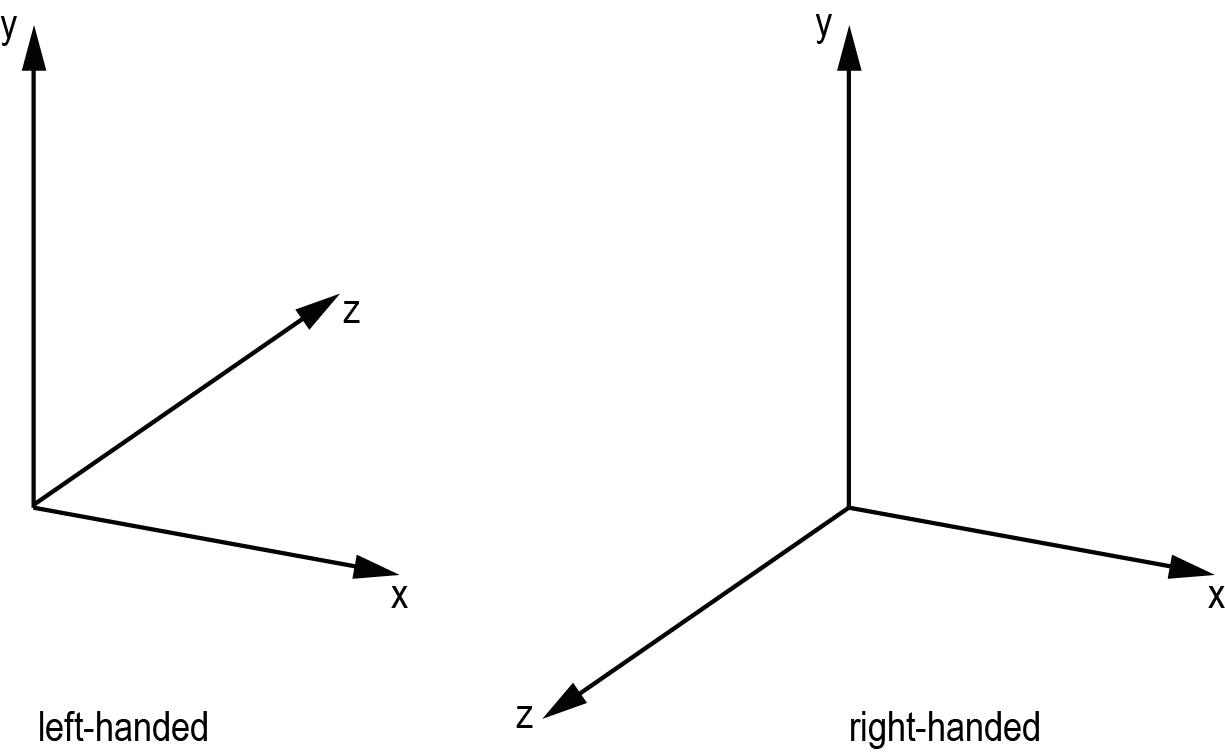
\includegraphics[width=0.8\textwidth]{figures/CoordinateSystems}
		\caption[Left- and right-handed Cartesian coordinate systems]{Left- and right-handed Cartesian coordinate systems (\textit{source: own illustration based on} \cite[p.167]{Gregory.2014}).}
		\label{fig:CoordinateSys}
\end{figure}

\subsection{Camera Models}
- projection from 3-D scene space onto a 2-D image plane
-camera mapping is represented by a matrix
-this matrix maps from homogeneous coordinates of a world point in 3-space to homogeneous coordinates of the imaged point on the image plane
-cameras properties, the internal camera parameters (intrinsics) are saved in another matrix K
-two important classes of cam matrices: finite cameras and cams with their centre at infinity, such as affine cam (represents parallel projection)
 (\cite[p.152]{Hartley.2011})
 
\subsubsection{Extrinsic parameters}
\subsubsection{Intrinsic paramters}

%------------------------------
\section{Epipolar Geometry}
%------------------------------
\subsection{Aufbau}
\subsection{Essential matrix}
\index{Essential matrix}
\subsection{Fundamental matrix}
\index{Fundamental matrix}
\enquote{In der Theorie benötigt der 8-Punkt-Algorithmus mindestens acht korrespondierende Punkte für die Berechnung der Fundamental-Matrix. Allerdings wird dabei eine hohe Genauigkeit der Werte vorausgesetzt. Bei einer manuellen Bestimmung der Punkte, hat es sich als sinnvoll herausgestellt, mehr als acht Korrespondezen zu wählen.}


%------------------------------
\section{3-D reconstruction}
%------------------------------

\subsection{Structure from motion}\label{ssec:SfM}
\subsection{Stereo matching}\label{ssec:stereoMatch}
 
\section{Disparity}

\begin{itemize}
\item Disparity Map
\end{itemize}

"Disparity refers to the distance between two corresponding points in the left and right image of a stereo pair. Obviously this process involves choosing a point in the left hand frame and then finding its match (often called the corresponding point) in the right hand image; often this is a particularly difficult task to do without making a lot of mistakes. A useful topic to read about when performing stereo matching is rectification. This will make the process of matching pixels in the left and right image considerably faster as the search will be horizontal."
(http://stackoverflow.com/questions/17607312/difference-between-disparity-map-and-disparity-image-in-stereo-matching)

\section{Rectification}
\section{Triangulation?}

\section{What else?}
\begin{itemize}
\item use Markus Mann - StereoCameraCalibration.pdf !!!!
\item and Camera Calibration for Stereo Vision.pdf
\item Levenberg-Marquardt algorithm? \url{http://www.cs.ubc.ca/~lowe/papers/danm96.pdf}
\item RANSAC?
\end{itemize}
